\documentclass{standalone}
\usepackage{standalone}

\begin{document}

\subsection{Matched Filter}
To detect the license plate, next step is to highlight plate like regions from the enhanced image. We used a mixture of Gaussian functions that emphasize the constancy of intensity along the horizontal direction of within the plate-like regions \cite{joarder2012bangla}. Equation \ref{eq:MixtureModel} shows the mathematical model of this function. This function can properly model low edge densities above, below and at the middle of the car plate. 

\begin{equation} \label{eq:MixtureModel}
h(x, y) = 
\begin{cases} 
	A.exp \left(
    	\dfrac{ -\left(x - \dfrac{m}{6} \right)^2 }
        	{ 0.2 \sigma_x^2 } \right),                                      
    	& \mbox{for } 
        	0 \leq x \leq \dfrac{m}{3}, 
            0 \leq y \leq n     
    \\ \vspace{0.2cm}
    B.exp \left( 
    	\dfrac{ -\left(x - 
        			\left( \dfrac{m}{3} + \dfrac{m}{6} \right) 
                \right)^2 }
        	{ 2 \sigma_x^2 } \right),                
        & \mbox{for }
        	\dfrac{m}{3} \leq x \leq 2\dfrac{m}{6}, 
        	0 \leq y \leq n 
    \\ \vspace{0.2cm}
    A.exp \left( 
    	\dfrac{ -\left(x - 
        			\left( 2\dfrac{m}{3} + \dfrac{m}{6} \right) 
                \right)^2 }
        	{ 0.2 \sigma_x^2 } \right),
    	& \mbox{for } 
        	2\dfrac{m}{3} \leq x \leq m, 
            0 \leq y \leq n         
\end{cases}
\end{equation}


In the Equation \ref{eq:MixtureModel}, 
$A$ and $B$ are coefficients of the mixture model. We set these parameters by observation and testing, following the condition: $A > 0$ and $B < 0$. The symbol $\sigma_x$ is the variance of the main lobe toward x direction. 
Figure \ref{fig:MixtureModelPlot} shows a plot depicting this equation.
\begin{figure} 
	\centering
	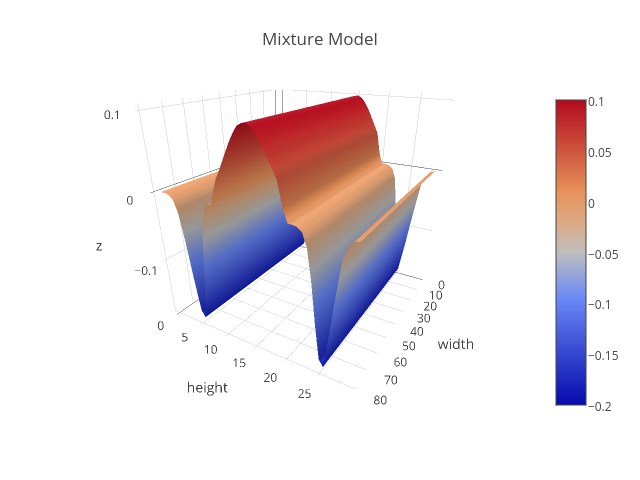
\includegraphics[width=.8\linewidth]{./img/plots/mixture.png}
	\caption{Matched Filter} 
	\label{fig:MixtureModelPlot}
\end{figure}

This filtering process provides a strong response at plate-like regions \cite{joarder2012bangla}\cite{Abolghasemi2009} (Figure \ref{fig:OriginalMixtureModel}). The result is compared against a threshold value, which is around $80\%$ of the maximum intensity. We call this process as smoothing, and the threshold value as {\it smoothing cutoff}.

\begin{figure}
\begin{subfigure}{.5\textwidth}
  \centering
  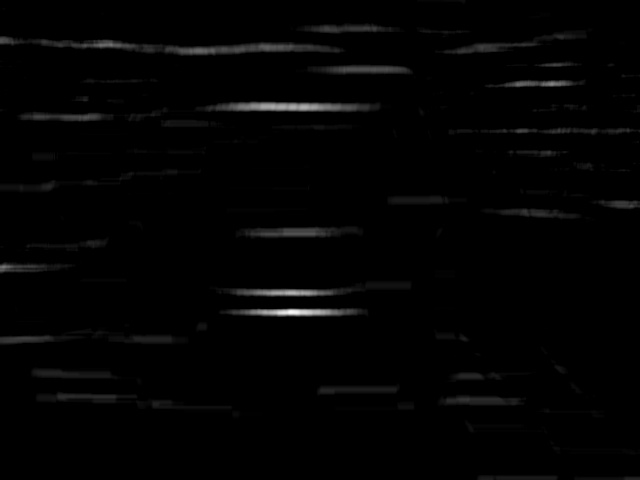
\includegraphics[width=.8\linewidth]{./img/sample/stage5-4.jpg}
  \caption{After applying the mixture model}
  \label{fig:OriginalMixtureModel}
\end{subfigure}
\begin{subfigure}{.5\textwidth}
  \centering
  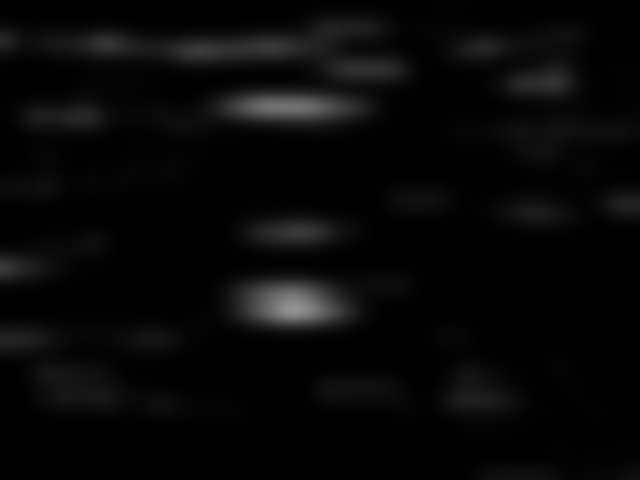
\includegraphics[width=.8\linewidth]{./img/sample/stage5-3.jpg}
  \caption{Gaussian blur on \ref{fig:OriginalMixtureModel}}
  \label{fig:BlurredMixtureModel}
\end{subfigure}
\begin{subfigure}{.5\textwidth}
  \centering
  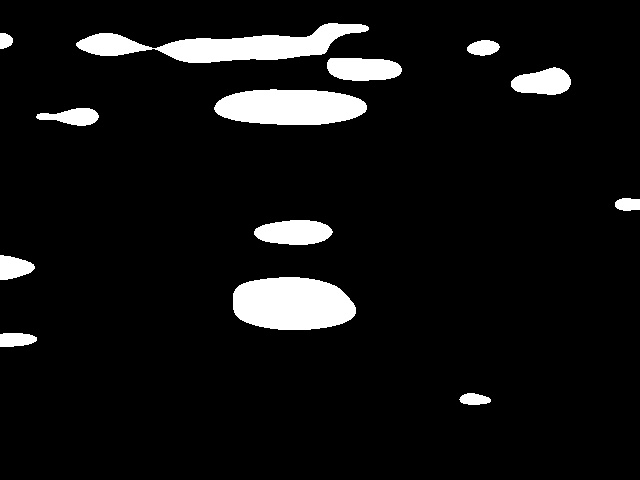
\includegraphics[width=.8\linewidth]{./img/sample/stage5-1.jpg}
  \caption{After applying adaptive threshold}
  \label{fig:ThresholdMixtureModel}
\end{subfigure}
\begin{subfigure}{.5\textwidth}
  \centering
  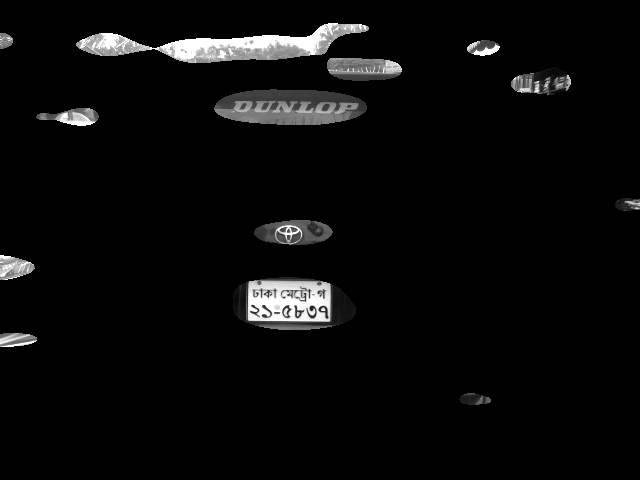
\includegraphics[width=.8\linewidth]{./img/sample/stage5-2.jpg}
  \caption{A see-through view of \ref{fig:ThresholdMixtureModel} with main image}
  \label{fig:GlassViewMixtureModel}
\end{subfigure}
\caption{Images after applying mixture model.}
\label{fig:MixtureModel}
\end{figure}


\end{document}